\documentclass[a4paper,14pt]{extarticle}

\usepackage[utf8x]{inputenc}
\usepackage[T1]{fontenc}
\usepackage[russian]{babel}
\usepackage{hyperref}
\usepackage{indentfirst}
\usepackage{here}
\usepackage{array}
\usepackage{graphicx}
\usepackage{caption}
\usepackage{subcaption}
\usepackage{chngcntr}
\usepackage{amsmath}
\usepackage{amssymb}
\usepackage[left=2cm,right=2cm,top=2cm,bottom=2cm,bindingoffset=0cm]{geometry}
\usepackage{multicol}
\usepackage{multirow}
\usepackage{titlesec}
\usepackage{listings}
\usepackage{color}
\usepackage{enumitem}
\usepackage{cmap}
\usepackage{url}

\definecolor{green}{rgb}{0,0.6,0}
\definecolor{gray}{rgb}{0.5,0.5,0.5}
\definecolor{purple}{rgb}{0.58,0,0.82}

\lstdefinelanguage{none}{}

\lstset{
	language={Python},
	backgroundcolor=\color{white},
	commentstyle=\color{green},
	keywordstyle=\color{blue},
	numberstyle=\color{gray}\scriptsize\ttfamily,
	stringstyle=\color{purple},
	basicstyle=\lst@ifdisplaystyle\footnotesize\fi\ttfamily,
	breakatwhitespace=false,
	breaklines=true,
	captionpos=b,
	keepspaces=true,
	numbers=left,
	numbersep=5pt,
	showspaces=false,
	showstringspaces=false,
	showtabs=false,
	tabsize=4,
	frame=single,
	morekeywords={},
	deletekeywords={},
	extendedchars=false,
	columns=fullflexible,
	literate=%
		{~}{{\raise.25ex\hbox{$\mathtt{\sim}$}}}{1}%
		{-}{-}{1}
}

\titleformat*{\section}{\large\bfseries}
\titleformat*{\subsection}{\normalsize\bfseries}
\titleformat*{\subsubsection}{\normalsize\bfseries}
\titleformat*{\paragraph}{\normalsize\bfseries}
\titleformat*{\subparagraph}{\normalsize\bfseries}

\counterwithin{figure}{section}
\counterwithin{equation}{section}
\counterwithin{table}{section}
\newcommand{\sign}[1][5cm]{\makebox[#1]{\hrulefill}}
\newcommand{\equipollence}{\quad\Leftrightarrow\quad}
\newcommand{\no}[1]{\overline{#1}}
\newcommand{\code}[1]{\lstinline[language=none]|#1|}
\graphicspath{{../pics/}}
\captionsetup{justification=centering,margin=1cm}
\def\arraystretch{1.3}
\setlength\parindent{5ex}
\titlelabel{\thetitle.\quad}

\setitemize{topsep=0em, itemsep=0em}
\setenumerate{topsep=0em, itemsep=0em}


\begin{document}

\begin{titlepage}
\begin{center}
	Санкт-Петербургский Политехнический Университет Петра Великого\\[0.3cm]
	Институт компьютерных наук и технологий \\[0.3cm]
	Кафедра компьютерных систем и программных технологий\\[4cm]

	\textbf{ОТЧЕТ}\\
	\textbf{по лабораторной работе}\\[0.5cm]
	\textbf{<<Поиск векторов смещения>>}\\[0.1cm]
	Разработка графических приложений\\[3.0cm]
\end{center}

\begin{flushright}
	\begin{minipage}{0.5\textwidth}
		\textbf{Работу выполнил студент}\\[3mm]
		гр. 3540901/91502 \hfill \sign[1.1cm] \hfill Дьячков В.В.\\[5mm]
		\textbf{Работу принял преподаватель}\\[5mm]
		\sign[5cm] \hfill Абрамов Н.А. \\[5mm]
	\end{minipage}
\end{flushright}

\vfill

\begin{center}
	Санкт-Петербург\\[0.3cm]
	\the\year
\end{center}
\end{titlepage}

\addtocounter{page}{1}


\tableofcontents
\newpage

\section{Программа работы}

Реализовать алгоритмы удаление шума из изображений при помощи:

\begin{enumerate}
	\item фильтра Гаусса;
	\item билатерального фильтра;
	\item NLM-фильтра.
\end{enumerate}

\section{Выполнение работы}

\subsection{Вспомогательные функции}

\paragraph{Зашумление изображения}

Исходное изображение, приведенное на рис \ref{fig:tower}, было зашумлено при помощи случайого шума с $\sigma = 10$. Зашумленное изображение, приведенное на рис \ref{fig:tower_noisy}, будет использоваться как исходное изображение для рассматриваемых фильтров. Результат работы фильтров будет сравниваться с оригинальным изображением.

\begin{lstlisting}[caption={Фунукция для добавления шума к изображению}]
def noised(img, sigma=1) :
	noise = np.random.normal(0, sigma, size=img.shape)
	return np.clip(img + noise, 0, 255).astype(np.uint8)
\end{lstlisting}

\begin{figure}[H]
	\centering
	\begin{subfigure}{0.48\linewidth}
		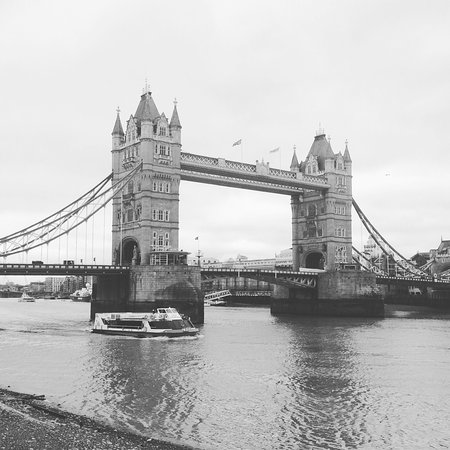
\includegraphics[width=\linewidth]{tower}
		\caption{Исходное изображение}
		\label{fig:tower}
	\end{subfigure}
	\begin{subfigure}{0.48\linewidth}
		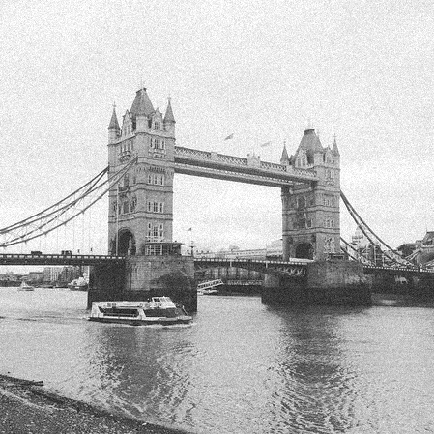
\includegraphics[width=\linewidth]{tower_noisy}
		\caption{Зашумленное изображение, $\sigma = 10$}
		\label{fig:tower_noisy}
	\end{subfigure}
	\caption{}
\end{figure}

\paragraph{Сравнение изображений}

Для сравнения получаемых изображений будем использовать сумму абсолютных разностей (sum of absolute differences, SAD). Для этого усредним разницу между соответствующими пикселями двух изображений.

\begin{lstlisting}[caption={Фунукция для сравнения изображений}]
def sad(a, b):
	return np.mean(np.abs(a.astype(np.float64) - b.astype(np.float64)))
\end{lstlisting}

Ориентиром является SAD между исходным и зашумленным изображениями -- $7.83$.

\subsection{Фильтр Гаусса}

В фильтре Гаусса (Gaussian blur) функция Гаусса применяется к исходному изображению для его размытия. Размытие изображение помогает уменьшить шум, но делает изображение нечетким. Функция Гаусса в одномерном и двумерном пространстве соответственно равна:

$$
G(x) = \dfrac{1}{\sqrt{2 \pi \sigma^2}} \exp{\left( -\dfrac{x^2}{2 \sigma ^2} \right)},
$$
$$
G(x, y) = \dfrac{1}{2 \pi \sigma^2} \exp{\left( -\dfrac{x^2 + y^2}{2 \sigma ^2} \right)}
$$

При помощи формулы Гаусса составляется матрица, которая затем используется как ядро свертки. Эта операция была подробно рассмотрена в предыдущей работе, поэтому используем для этого готовую функцию библиотеки OpenCV -- \code{cv.filter2D}.

\begin{lstlisting}[caption={Фунукция для применения фильтра Гаусса}]
def gaussian(v, sigma):
	return np.exp(-(v ** 2) / (2 * sigma ** 2)) / np.sqrt(2 * math.pi * sigma)
	
def gauss(x, y, sigma):
	return math.exp(-(x ** 2 + y ** 2) / (2 * sigma ** 2)) / (2 * math.pi * sigma)
	
def gauss_kernel(sigma, size=None):
	K = round(4 * sigma + 1) if size is None else size
	kernel = np.zeros((K, K))
	for i in np.arange(K):
		for j in np.arange(K):
			kernel[i, j] = gauss(i - K // 2, j - K // 2, sigma)
	return kernel / kernel.sum()
	
def gauss_filter(img, sigma):
	return cv.filter2D(img, 0, gauss_kernel(sigma))
\end{lstlisting}

Фильтр имеет единственный параметр -- $\sigma$. Будем варьировать его значение в пределах $0.2 \div 2.8$ с шагом $0.2$.

\begin{table}[H]
	\centering
	\caption{Зависимость SAD в зависимости от $\sigma$}
	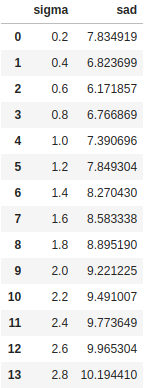
\includegraphics[scale=0.7]{tower_gauss_sad}
\end{table}

Визуализизируем значение SAD в зависимости от $\sigma$.

\begin{figure}[H]
	\centering
	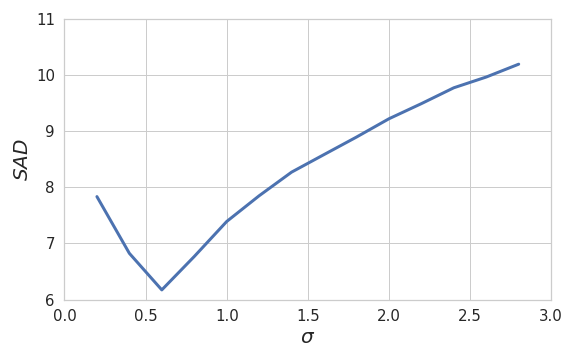
\includegraphics[width=0.75\linewidth]{tower_gauss_tune}
	\caption{Зависимость SAD в зависимости от $\sigma$}
\end{figure}

Оптимальным значением оказалось $\sigma = 0.6$.

\begin{figure}[H]
	\centering
	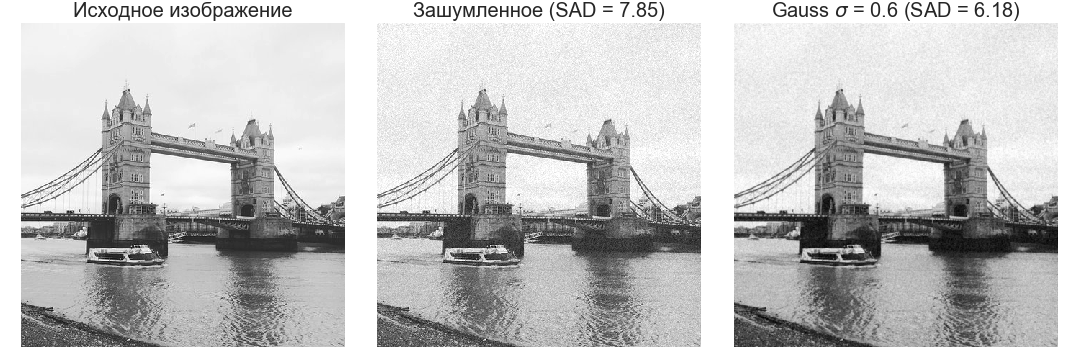
\includegraphics[width=\linewidth]{tower_gauss}
	\caption{Применение фильтра Гаусса при оптимальных параметерах}
\end{figure}

Сравним результат применения фильтра при разных значениях $\sigma$.

\begin{figure}[H]
	\centering
	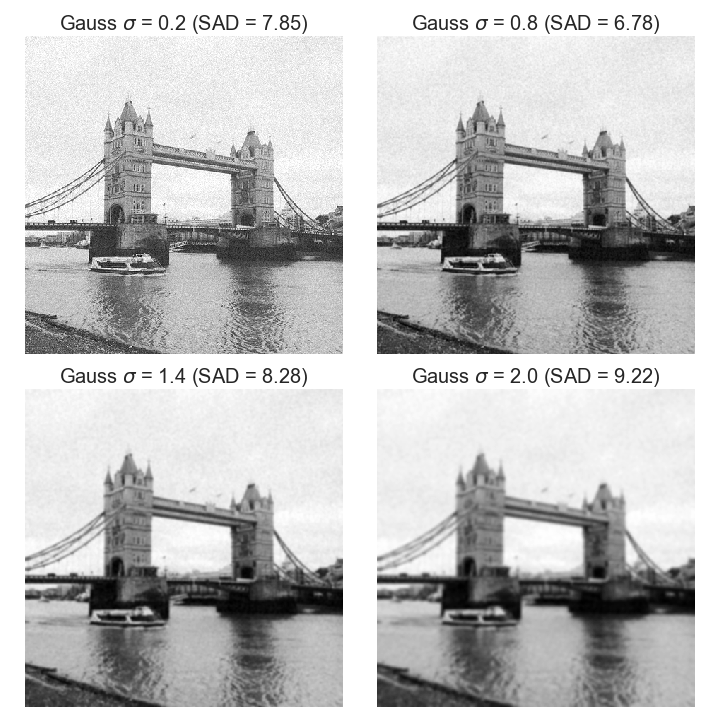
\includegraphics[width=0.8\linewidth]{tower_gauss_compare}
	\caption{Применение фильтра Гаусса при разных параметрах}
\end{figure}

Видно, что, чем больше значение $\sigma$, тем более размытым получается изображение.

\newpage

\subsection{Билатеральный фильтр}

Билатеральный фильтр -- нелинейный фильтр, выполняющий пространственное усреднение в пределах своей маски. Он может быть выбран в качестве эффективной техники удаления шума и ряда других искажающих факторов. Важным вопросом при работе с билатеральным фильтром является выбор его параметров, которые влияют на эффективность фильтрации.

Билатеральный фильтр определяется следующей формулой:
$$
I^{\text{filtered}}(x, \sigma_s, \sigma_r)={\frac {1}{W_{p}}}\sum _{x_{i}\in \Omega }I(x_{i}) \cdot f_{r}(\|I(x_{i})-I(x)\|, \sigma_r) \cdot g_{s}(\|x_{i}-x\|, \sigma_s),
$$
$$
W_{p}=\sum _{x_{i}\in \Omega }{f_{r}(\|I(x_{i})-I(x)\|) \cdot g_{s}(\|x_{i}-x\|)}
$$

Параметры фильтра $\sigma_s$ и $\sigma_r$ отвечают за формирование весов. Они определяют максимальные значения производных соответствующих Гауссовых весовых функций и, следовательно, служат порогами для процедуры идентификации пикселей, близких друг к другу пространственно или радиометрически. В случае $\sigma_s \rightarrow \infty$ соответствующий фильтр стремится к линейному фильтру Гаусса с дисперсией $\sigma$, а в случае, $\sigma_r\ \sigma_r \rightarrow \infty$ -- к усредняющему фильтру. Билатеральный фильтр успешно используется в системах обработки изображений для удаления Гауссова шума.

Немаловажным параметром билатерального фильтра является размер маски. Он связан с пространственным фильтром Гаусса. Обычно, основываясь на свойстве распределения Гаусса, размер окна выбирают в пределах 2-3 стандартных отклонений Гаусса. В реализованном фильтре используется $2 \sigma_s + 1$ пикселей в каждую из сторон от текущего пикселя.

\begin{lstlisting}[caption={Фунукция для применения билатерального фильтра}]
def bilateral_filter(img, sigma_s, sigma_r):
	n_neig = sigma_s * 2 + 1
	result = np.zeros_like(img, dtype=np.float64)
	img_pad = np.pad(img, n_neig, mode='reflect').astype(np.float64)
	for i in range(n_neig, img.shape[0] + n_neig):
		for j in range(n_neig, img.shape[1] + n_neig):
			region = img_pad[(i - n_neig) : (i + n_neig + 1), (j - n_neig) : (j + n_neig + 1)]
			space_weights = gauss_kernel(sigma_s, size=(n_neig * 2 + 1))
			range_weights = gaussian(region - img_pad[i, j], sigma_r)
			weights = space_weights * range_weights
			result[i - n_neig, j - n_neig] = np.sum(region * weights) / weights.sum()
	return np.clip(result, 0, 255).astype(np.uint8)
\end{lstlisting}

Будем варьировать значения $\sigma_r$ и $\sigma_r$ в пределах $1 \div 10$ с шагом $3$.

\begin{table}[H]
	\centering
	\caption{Зависимость SAD в зависимости от $\sigma_s$ и $\sigma_r$}
	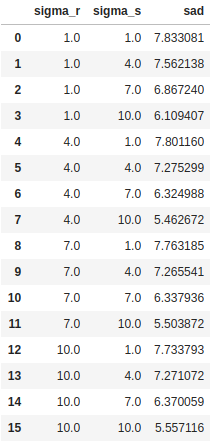
\includegraphics[scale=0.7]{tower_bilateral_sad}
\end{table}

Визуализизируем значение SAD в зависимости от $\sigma_r$ и $\sigma_r$.

\begin{figure}[H]
	\centering
	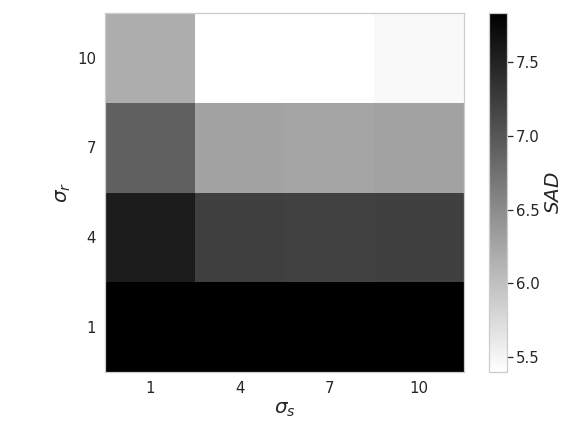
\includegraphics[width=0.75\linewidth]{tower_bilateral_tune}
	\caption{Зависимость SAD в зависимости от $\sigma_r$ и $\sigma_r$}
\end{figure}

Очевидно, что чем больше размер окон (которые зависят от $\sigma_s$ и $\sigma_r$), тем лучше фильтр удаляет шум. Однако при этом возрастает время работы фильтра, поэтому $\sigma > 10$ не были рассмотрены. Оптимальными значениями фильтра оказались $\sigma_s = 10$ и $\sigma_r = 4$.

\begin{figure}[H]
	\centering
	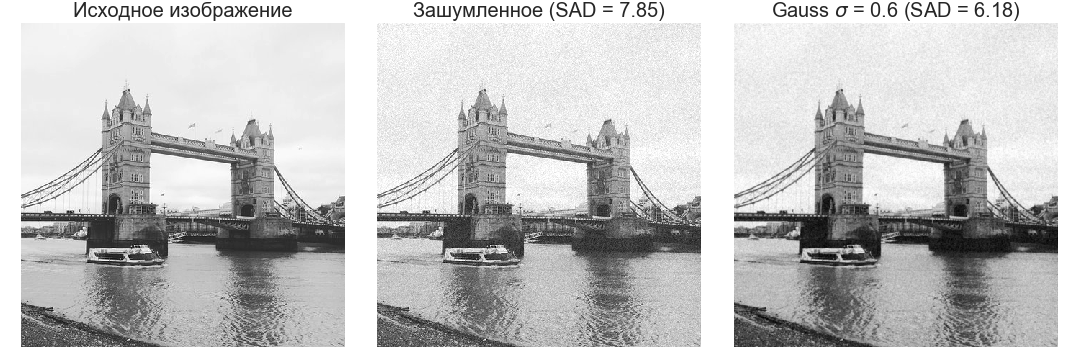
\includegraphics[width=\linewidth]{tower_bilateral}
	\caption{Применение билатерального фильтра при оптимальных параметрах}
\end{figure}

\subsection{NLM-фильтр}

Non-local means (NLM) -- нелинейный фильтр, используемый в обработке изображений для удаления шума из изображения. В отличии от <<локальных>> фильтров, которые берут среднее значение группы пикселей, окружающих текущий пиксель, NLM использует среднее значение всех пикселей в некотором большем окне. Дополнительно в NLM окружающие пиксели взвешиваются в зависимости от похожести на текущий. Данный факт позволяет избежать потери деталей на изображении.

NLM-фильтр определяется следующей формулой:
$$
u(p)={1 \over C(p)}\sum _{{q\in \Omega }}v(q)f(p,q),
$$
$$
C(p)=\sum _{{q\in \Omega }}f(p,q)
$$

Рассмотрим параметры фильтра:
\begin{itemize}
	\item $\sigma_r$ -- параметр, аналогичный билатеральному фильтру, и отвечающий за формирование весов
	\item $N_{comp}$ -- размер окна, в котором происходит поиск похожим пикселей
	\item $N_{neig}$ -- размер окна, которое используется для сравнения схожести окрестностей двух пикселей
\end{itemize}

\newpage

\begin{lstlisting}[caption={Фунукция для применения билатерального фильтра}]
def nlm_local(img, x, y, sigma_r, n_comp, n_neig):
	height, width = img.shape
	value, wp = 0, 0
	
	values = img[(x - n_neig):(x + n_neig + 1), (y - n_neig):(y + n_neig + 1)]
	template = img[(x - n_comp):(x + n_comp + 1), (y - n_comp):(y + n_comp + 1)]
	weight = lambda x: gaussian(sad(template, x), sigma_r)
	
	weights = np.reshape([
		weight(img[(i - n_comp) : (i + n_comp + 1), (j - n_comp) : (j + n_comp + 1)]) \
			for i in np.arange(x - n_neig, x + n_neig + 1) \
			for j in np.arange(y - n_neig, y + n_neig + 1)], values.shape)
	res = np.sum(values * weights) / weights.sum()
	return res
	
def nlm_filter(img, sigma_r, n_comp, n_neig):
	n_comp_half = n_comp // 2
	n_neig_half = n_neig // 2
	pad = n_comp_half + n_neig_half
	img_pad = np.pad(img, pad, mode='reflect').astype(np.float64)
	result = np.zeros_like(img, np.float64)
	for i in np.arange(pad, img.shape[0] + pad):
		for j in np.arange(pad, img.shape[1] + pad):
			result[i - pad, j - pad] = nlm_local(img_pad, i, j, sigma_r, n_comp_half, n_neig_half)
	return np.clip(0, 255, result).astype(np.uint8)
\end{lstlisting}

Будем варьировать параметры в разумных пределах, приведенных в таблице ниже.

\begin{table}[H]
	\centering
	\begin{subfigure}{0.48\linewidth}
		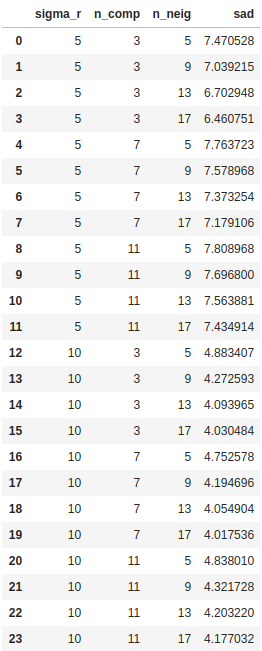
\includegraphics[scale=0.7]{tower_nlm_sad}
	\end{subfigure}
	\begin{subfigure}{0.48\linewidth}
		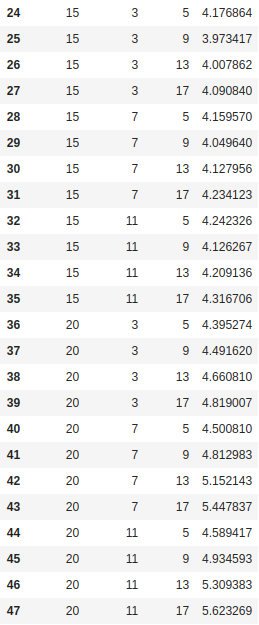
\includegraphics[scale=0.7]{tower_nlm_sad_2}
	\end{subfigure}
	\caption{Зависимость SAD в зависимости от $\sigma_r$, $ N_{comp}$ и $N_{neig}$}
\end{table}

Визуализизируем значение SAD в зависимости от $N_{comp}$ и $N_{neig}$ при фиксированном значении $\sigma_r = 15$.

\begin{figure}[H]
	\centering
	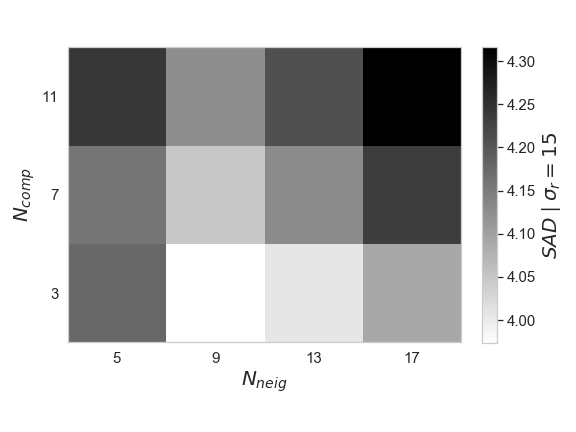
\includegraphics[width=0.75\linewidth]{tower_nlm_tune}
	\caption{Зависимость SAD в зависимости от $\sigma_r$ и $\sigma_r$}
\end{figure}

Оптимальными значениями фильтра оказались $\sigma_r = 15$, $N_{comp} = 3$ и $N_{neig} = 9$.

\begin{figure}[H]
	\centering
	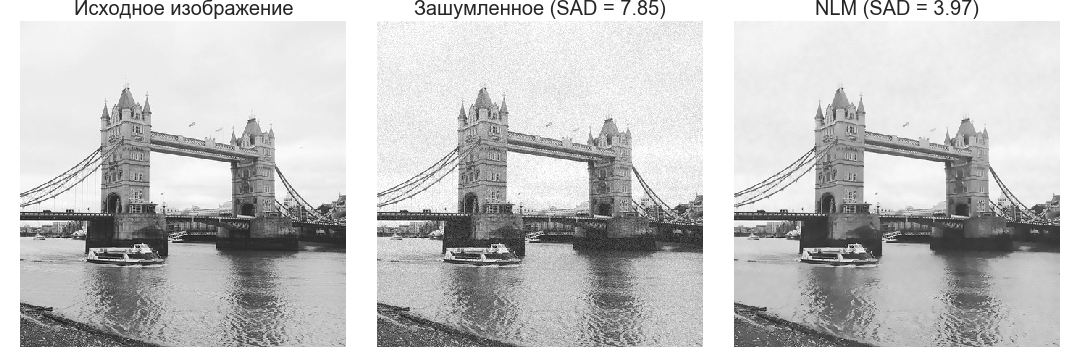
\includegraphics[width=\linewidth]{tower_nlm}
	\caption{Применение NLM-фильтра при оптимальных параметрах}
\end{figure}

\subsection{Сравнение фильтров}

Сравним результаты применения фильтров с оптимальными параметрами к зашумленному изображению.

\begin{figure}[H]
	\centering
	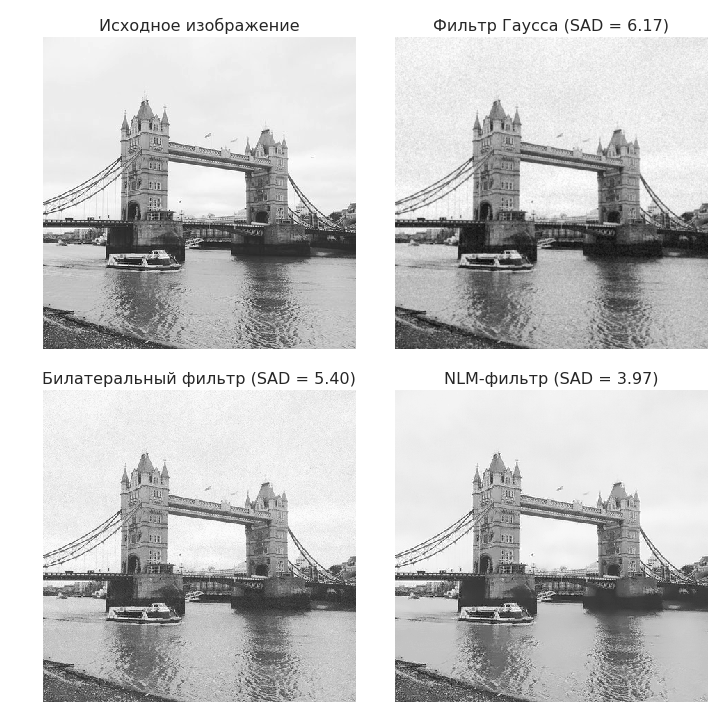
\includegraphics[width=0.9\linewidth]{tower_compare}
	\caption{Сравнение применения реализованных фильтров}
\end{figure}

\section{Выводы}

В данной работе были реализованы три фильтра для удаление шума из изображений:

\begin{itemize}
	\item фильтр Гаусса;
	\item билатеральный фильтр;
	\item NLM-фильтр.
\end{itemize}

Из получившихся изображений и значений SAD видно, что лучше других себя проявил NLM-фильтр. Заметный шум был удален из изображения, при этом были сохранены мелкие детали изображения. Хуже других оказался фильтр Гаусса, что объясняется его простой (взвешенное усреднение окрестности). Билатеральный фильтр удалил из изображения большую часть шума и может быть также использован для избавления шума из изображений.

\end{document}
